\chapter{Parallelizzazione con OpenMP}
\label{cap:openmp}

\section{L'Approccio della Versione d'Esame}

OpenMP~\cite{openmp} permette di parallelizzare un programma C annotandolo con direttive \codice{\#pragma omp}, che il compilatore traduce in codice multi-thread quando si compila con l'opzione \codice{-fopenmp}. La versione d'esame manteneva l'algoritmo originale, con le interrogazioni intrecciate all'espansione, e cercava il parallelismo all'interno della singola interrogazione:

\begin{itemize}
    \item la visita ricorsiva del Ball Tree apriva una regione \codice{parallel sections} per esplorare in parallelo i due figli di ogni nodo;
    \item la scansione di una foglia era un ciclo \codice{parallel for}, con una sezione \codice{critical} attorno a ogni inserimento di un punto nel risultato;
    \item l'assegnazione dell'etichetta ai punti di un intorno era a sua volta un ciclo \codice{parallel for}.
\end{itemize}

L'approccio aveva tre problemi. Il primo è che non è mai stato eseguito: gli script di compilazione della cartella OpenMP non passavano l'opzione \codice{-fopenmp}, il compilatore ignorava le direttive, e il binario a 32 bit \enquote{con OpenMP} risultava identico byte per byte a quello senza. Il secondo è la granularità: una interrogazione dura pochi microsecondi, meno del costo di creare e sincronizzare un gruppo di thread, e ogni livello della ricorsione ne apriva uno nuovo; la sezione critica serializzava poi proprio gli inserimenti. Il terzo è la misura: il tempo era calcolato con \codice{clock()}, che restituisce il tempo di CPU del processo, cioè la somma dei tempi di tutti i thread, e che con più thread cresce anche quando il programma diventa più veloce. La relazione d'esame dichiarava infatti di non poter misurare il beneficio di OpenMP.

\section{Parallelizzazione della Prima Fase}

La formulazione in due fasi (Sezione~\ref{sec:due-fasi}) sposta il parallelismo al livello più alto possibile: le $n$ interrogazioni della prima fase sono indipendenti e vengono distribuite tra i thread con un unico ciclo parallelo (Figura~\ref{fig:fasi}).

\begin{lstlisting}[language=C, caption={La prima fase in \codice{src/dbscan.c}, semplificata.}, label={lst:fase1}]
#pragma omp parallel reduction(+ : evals, kept, core_points)
{
    PointList found; // riusata da tutte le interrogazioni del thread
    point_list_init(&found, 256);
#pragma omp for schedule(dynamic, 64)
    for (int p = 0; p < n; p++) {
        point_list_clear(&found);
        evals += ball_tree_query(&tree, ds, p, eps, dist2, &found);
        is_core[p] = found.size + 1 >= min_pts;
        if (is_core[p])
            neighbours[p] = copia di found.items;
    }
    point_list_free(&found);
}
\end{lstlisting}

\begin{figure}[H]
    \centering
    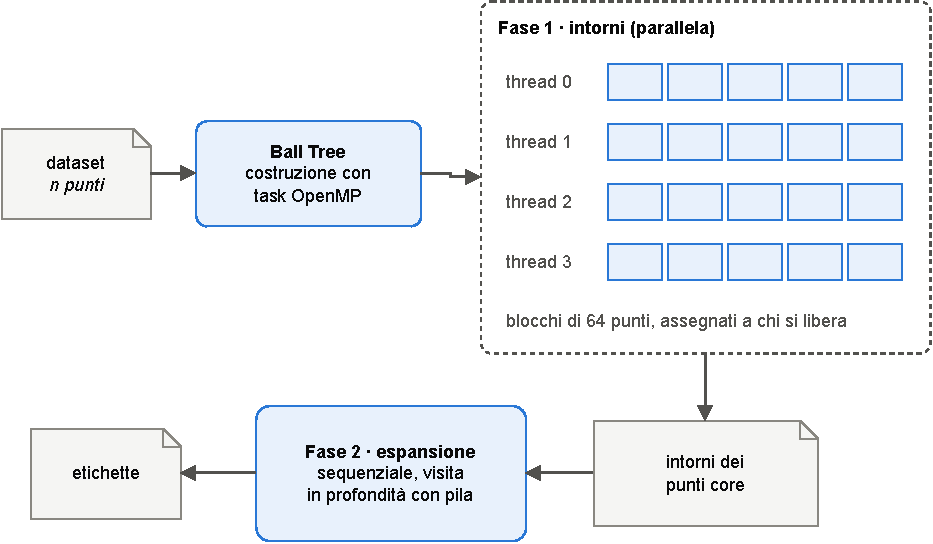
\includegraphics[width=\textwidth]{diagrammi/fasi.pdf}
    \caption{Le due fasi dell'algoritmo: la costruzione del Ball Tree e le interrogazioni sono parallele, l'espansione dei cluster è sequenziale.}
    \label{fig:fasi}
\end{figure}

Le scelte principali sono tre:

\begin{itemize}
    \item \textbf{nessuna sincronizzazione nel ciclo}: ogni iterazione scrive solo nelle celle di indice $p$ dei vettori \codice{is\_core}, \codice{count} e \codice{neighbours}, e ogni thread ha la propria lista temporanea. I contatori statistici sono sommati con una clausola \codice{reduction};
    \item \textbf{assegnazione dinamica}: il costo di un'interrogazione varia molto da punto a punto, perché un punto al centro di un cluster ha molti vicini e un punto isolato quasi nessuno. Con \codice{schedule(dynamic, 64)} i thread prelevano blocchi di 64 punti man mano che si liberano, invece di ricevere in anticipo una porzione fissa, e il carico si bilancia da sé. Il blocco di 64 punti rende trascurabile il costo della distribuzione;
    \item \textbf{ordine indipendente dai thread}: ogni intorno contiene sempre gli stessi punti, e la seconda fase li legge in ordine di indice. Il risultato è quindi identico con qualunque numero di thread, come verificano i test.
\end{itemize}

\section{Costruzione Parallela del Ball Tree}

La costruzione del Ball Tree è ricorsiva e i due sottoalberi di un nodo sono indipendenti, perché occupano intervalli disgiunti del vettore \codice{order}. Ogni chiamata ricorsiva diventa quindi un \emph{task} OpenMP, creato all'interno di una regione parallela da un solo thread (\codice{single}) ed eseguito da un thread qualunque del gruppo; \codice{taskwait} attende i due figli prima di restituire il nodo. Sotto i 4096 punti la clausola \codice{if} esegue il sottoalbero direttamente, perché un task così piccolo costerebbe più di quanto fa risparmiare. Il guadagno è limitato dal fatto che la suddivisione della radice, che esamina tutti i punti, è necessariamente eseguita da un solo thread; la costruzione pesa comunque circa l'1\% del tempo totale.

\section{Perché l'Espansione Resta Sequenziale}

La seconda fase non calcola distanze: visita un grafo i cui archi sono già noti, con un costo proporzionale alla somma delle dimensioni degli intorni. Nelle misure pesa tra lo 0,2\% e l'1\% del tempo totale, secondo il numero di thread, quindi parallelizzarla porterebbe un beneficio trascurabile. Sarebbe anche difficile farlo senza cambiare il risultato: due thread che espandono cluster diversi possono contendersi un punto di confine, e l'assegnazione al primo cluster che lo raggiunge richiede un ordine di visita definito. Una versione parallela dovrebbe calcolare le componenti connesse dei punti core con una struttura \emph{union-find} e assegnare i punti di confine in un passo successivo (Capitolo~\ref{cap:limiti}).

\section{Misura del Tempo}

Il programma misura il tempo reale trascorso, con la funzione \codice{clock\_gettime} e l'orologio monotono del sistema, separatamente per la costruzione dell'indice, la prima e la seconda fase. Il tempo riportato comprende solo il clustering e non la lettura del file, come nella versione d'esame, così che le due siano confrontabili. Per la versione d'esame, che è sequenziale, il tempo di CPU misurato da \codice{clock()} coincide in pratica con il tempo reale.
